\documentclass{article}
\usepackage{graphicx}
\usepackage{amsmath}
\usepackage{pgfplots}
\usepackage{physics}
\usepackage{cancel}
\usepackage{enumitem}
\usepackage{txfonts}

\pgfplotsset{compat=1.18}

\newcommand{\Eth}{E_{\text{th}}}

\usepackage[a4paper, top=1cm, bottom=2cm, left=2cm, right=2cm, includehead, includefoot]{geometry}

\begin{document}

\noindent
Physics 4A - Classical Mechanics \hfill Prof. Roger King

\noindent\rule{\textwidth}{0.4pt}

\begin{center}
    \textbf{\LARGE Homework 12} \\
    \vspace{12pt}
    \large Aaron W. Tarajos \\
    \textit{\today}
\end{center}

\noindent\rule{\textwidth}{0.4pt}

\section*{Problem 1}
In 1932, James Chadwick fired neutrons of unknown speed and mass into different
substances. He found that protons (of mass 1 $u$) were given a speed 7.5 times that given to
nitrogen nuclei (of mass 14 $u$). If the collisions were elastic and head on, what can you deduce
about the mass of the neutron?

\subsection*{Solution}
The neutron must also have a mass of $1u$. Let $n$ denote the neutron, $p$ denote the proton, and $N$ denote the Nitrogen;
\begin{align*}
	\frac{v_p}{v_N} &= \frac{2 m_n}{m_n + m_p} \cdot \frac{m_n + m_N}{2m_n} \\
	\frac{7.5 v_N}{v_N} &= \frac{m_n + m_N}{m_n + m_p} \\
	7.5m_n + 7.5m_p &= m_n + m_N \\
	m_n &= \frac{m_N - 7.5m_p}{6.5} \\
	m_n &= \frac{14 - 7.5}{6.5} \\
	m_n &= \boxed{1\ u}
\end{align*}

\section*{Problem 2}
2) A one-dimensional inelastic collision may be characterized by a coefficient of restitution $e$
that relates the relative velocities before and after the collision: $\left(v_{1,f} - v_{2,f}\right) = -e\left(v_{1,i} - v_{2,i} \right)$
Show that the final velocities are:
\[
	v_{1,f} = \frac{(m_1 - e m_2)v_{1,i} + m_2 (1+e)v_{2,i}}{m_1 + m_2}
\]
\[
	v_{2,f} = \frac{(m_2 - e m_1)v_{2,i} + m_1 (1+e)v_{1,i}}{m_1 + m_2}
\]
(Hint, kinetic energy is not conserved. You will need two equations so solve for the two
unknowns.)

\subsection*{Solution}
Given the conservation of momentum;

\[
	m_1v_{1i} + m_2v_{2i} = m_1v_{1f} + m_2v_{2f}
\]
and the restitution equations, let

\[
	v_{2f} = v_{1f} + e(v_{1i}-v_{2i})
\]
then
\begin{align*}
	m_1 v_{1,i} + m_2 v_{2,i} &= m_1 v_{1,f} + m_2 \left[ v_{1,f} + e (v_{1,i} - v_{2,i}) \right] \\
	 &= m_1 v_{1,f} + m_2 v_{1,f} + m_2 e (v_{1,i} - v_{2,i}) \\
	 &= (m_1 + m_2) v_{1,f} + m_2 e (v_{1,i} - v_{2,i}) \\
	 &= m_1 v_{1,i} + m_2 v_{2,i} - m_2 e v_{1,i} + m_2 e v_{2,i} \\
	 &= (m_1 v_{1,i} - m_2 e v_{1,i}) + (m_2 v_{2,i} + m_2 e v_{2,i}) \\
	 &= \left[ m_1 - m_2 e \right] v_{1,i} + m_2 (1 + e) v_{2,i} \\
	(m_1 + m_2) v_{1,f} &= \left[ m_1 - m_2 e \right] v_{1,i} + m_2 (1 + e) v_{2,i} \\
	v_{1,f} &= \frac{ (m_1 - m_2 e) v_{1,i} + m_2 (1 + e) v_{2,i} }{ m_1 + m_2 }
\end{align*}
Then for the other equation, start with $v_{2,f}$

\[
v_{2,f} = v_{1,f} + e (v_{1,i} - v_{2,i})
\]
and substitute \( v_{1,f} \);

\begin{align*}
	v_{2,f} &= \frac{ (m_1 - m_2 e) v_{1,i} + m_2 (1 + e) v_{2,i} }{ m_1 + m_2 } + e (v_{1,i} - v_{2,i}) \\
&= \frac{(m_1 - m_2 e) v_{1,i} + m_2 (1 + e) v_{2,i} + (m_1 + m_2) e v_{1,i} - (m_1 + m_2) e v_{2,i}} { m_1 + m_2 }\\
&= \frac{[m_1 - m_2 e + m_1 e + m_2 e] v_{1,i} + [m_2 (1 + e) - (m_1 + m_2) e] v_{2,i}} { m_1 + m_2 }\\
&= \frac{[m_1 (1 + e)] v_{1,i} + [m_2 + m_2 e - m_1 e - m_2 e] v_{2,i}} { m_1 + m_2 }\\
&= \frac{[m_1 (1 + e)] v_{1,i} + [m_2 - m_1 e] v_{2,i}} { m_1 + m_2 }\\
	v_{2,f} &= \frac{ m_1 (1 + e) v_{1,i} + (m_2 - m_1 e) v_{2,i} }{ m_1 + m_2 }
\end{align*}


\section*{Problem 3}
An alpha particle ($^4$He) undergoes an elastic collision with a stationary uranium nucleus ($^235$U). What
percent of the kinetic energy of the alpha particle is transferred to the uranium nucleus? Assume the
collision is one dimensional.

\subsection*{Solution}
We find the uranium nucleus final velocity to be
\[
v_{2f} = \left( \frac{2 m_1}{m_1 + m_2} \right) v_{1i}
\]
and the final kinetic energy to be
\[
K_{2f} = \frac{1}{2} m_2 v_{2f}^2
\]
Substitute \( v_{2f} \):

\begin{align*}
K_{2f} &= \frac{1}{2} m_2 \left( \frac{2 m_1}{m_1 + m_2} v_{1i} \right)^2 \\
	&= \frac{1}{2} m_2 \left( \frac{4 m_1^2 v_{1i}^2}{(m_1 + m_2)^2} \right) \\
	&= \left( \frac{2 m_2 m_1^2 v_{1i}^2}{(m_1 + m_2)^2} \right)
\end{align*}
and the ratio of final kinetic energy for the uranium and initial kinetic energy of the alpha particle is;
\begin{align*}
	\frac{K_{2f}}{K_{1i}} &= \left( \frac{2 m_2 m_1^2 v_{1i}^2}{(m_1 + m_2)^2} \right) \cdot \frac{2}{m_1v_{1i}^2} \\
	&= \frac{4 m_2 m_1^2 v_{1i}^2}{(m_1 + m_2)^2 m_1v_{1i}^2} \\
	&= \frac{4 m_1 m_2}{(m_1 + m_2)^2} \\
	&= \frac{4(235)(4)}{(4+235)^2} \\
	&= \frac{3760}{57121} \\
	&= \boxed{6.581\ \%}
\end{align*}

\section*{Problem 4}
A steel ball of mass 0.500 kg is fastened to a cord that is 70.0 cm long and fixed at the far end. The
ball is then released when the cord is horizontal. At the bottom of its path, the ball strikes a 2.50 kg steel
block initially at rest on a frictionless surface. The collision is elastic. Find (a) the speed of the ball and
(b) the speed of the block, both just after the collision.

\begin{figure}[ht]
    \centering
    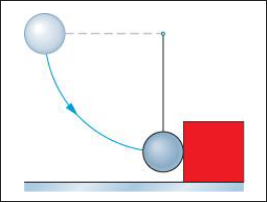
\includegraphics[scale=0.5]{drawing-1.png}
\end{figure}

\subsection*{Solution}
\subsubsection*{Part a:}
The initial velocity with which the ball strikes the block is given by;
\[
	v_{1,i} = \sqrt{2g \delta y}
\]
Then we can solve for the final velocity
\begin{align*}
	v_{1,f} &= \frac{m_1 - m_2}{m_1 + m_2} v_{1,i} \\
		&= \frac{m_1 - m_2}{m_1 + m_2} \sqrt{2g \delta y} \\
		&= \frac{0.500 - 2.50}{0.500 + 2.50} \sqrt{2 (9.81)(0.70)} \\
		&= -2.471\ \text{m}/\text{s}
\end{align*}
then speed is $|v_{1,f}|$;

\[
	\boxed{s_{1,f} = 2.47\text{m}/\text{s}}
\]

\subsubsection*{Part b:}
The velocity of the block is given by;
\begin{align*}
	v_{2,f} &= \frac{2 m_1}{m_1 + m_2}v_{1,i} \\
		&= \frac{2 m_1}{m_1 + m_2} \sqrt{2g \delta y} \\
		&= \frac{2(0.50)}{0.50 + 2.50} \sqrt{2(9.81)(0.70)} \\
		&= 1.235\ \text{m}/\text{s}
\end{align*}
Similarly the speed is given by $|v_{2,f}|$;

\[
	\boxed{s_{2,f} = 1.235\ \text{m}/\text{s}}
\]

\section*{Problem 5}
The platter in a belt drive turntable is driven by a belt that wraps around a hub, of radius 3.00
cm, below the platter and around the shaft of the motor. If the platter rotates at 33.3 rpm and the
motor rotates at 60 rpm, what is the required radius of the shaft?

\subsection*{Solution}
The tangential velocities must be the same, therefore;
\begin{align*}
	\omega_h r_h &= \omega_s r_s \\
	r_s &= \frac{\omega_h r_h}{\omega_s} \\
	r_s &= \frac{33.3 \cdot 3}{50} \\
	r_s &= \boxed{1.665\ \text{cm}}
\end{align*}

\section*{Problem 6}
At $t = 0$, a flywheel has an angular velocity of 4.70 rad/s, a constant angular acceleration of
-0.24 rad/s$^2$, and a reference line at $\theta_0 = 0$. (a) Through what maximum angle $\theta_{\text{max}}$ will the
reference line turn in the positive direction? What are the (b) first and (c) second times the
reference line will be at $\theta = \frac{1}{2}\theta_\text{max}$? At what (d) negative time and (e) positive time will the
reference line be at $\theta$ = -10.5 rad? (f) Graph $\theta$ versus $t$, and indicate your answers.

\subsection*{Solution}
\subsubsection*{Part a:}
The maximum angle theta occurs where $\omega = 0$.
\begin{align*}
	\omega^2 &= \omega_0^2 + 2\alpha(\delta \theta) \\
	\theta &= \frac{\omega^2 - \omega_0^2}{2 \alpha} \\
	\theta &= \frac{0^2 - 4.70^2}{2(-0.24)} \\
	       &= \boxed{46.021\ \text{rad}}
\end{align*}
\subsubsection*{Part b and c:}
The two times that the reference line will be at $\frac{1}{2}\theta_\text{max}$ is given by
\begin{align*}
	\Delta \theta &= \omega_0 t + \frac{1}{2}\alpha t^2 \\
	t &= \frac{-\omega_0 \pm \sqrt{\omega_0^2 - 4(\alpha/2)(-\theta)}}{2(\alpha/2)} \\
	  &= \frac{-\omega_0 \pm \sqrt{\omega_0^2 + 2 \alpha \theta}}{\alpha} \\
	  &= \frac{-4.70 \pm \sqrt{4.7^2 + (2)(-0.24)(23.01)}}{-0.24}
\end{align*}
then

\[
	\boxed{t_1 = 5.736\ \text{s} \quad \text{and} \quad t_2 = 33.431\ \text{s}}
\]

\subsubsection*{Part d and e:}
Given $\theta = -10.5$ we can solve for the positive and negative time using the same equation as the previous parts;
\begin{align*}
	t &= \frac{-\omega_0 \pm \sqrt{\omega_0^2 + 2 \alpha \theta}}{\alpha} \\
	  &= \frac{-4.70 \pm \sqrt{4.7^2 + (2)(-0.24)(-10.5)}}{-0.24}
\end{align*}
giving us a negative time;
\[
	\boxed{t_1 = -2.119\ \text{s}}
\]
and a postive time;
\[
	\boxed{t_2 = 41.286\ \text{s}}
\]

\subsubsection*{Part f:}
\begin{figure}[!ht]
    \centering
    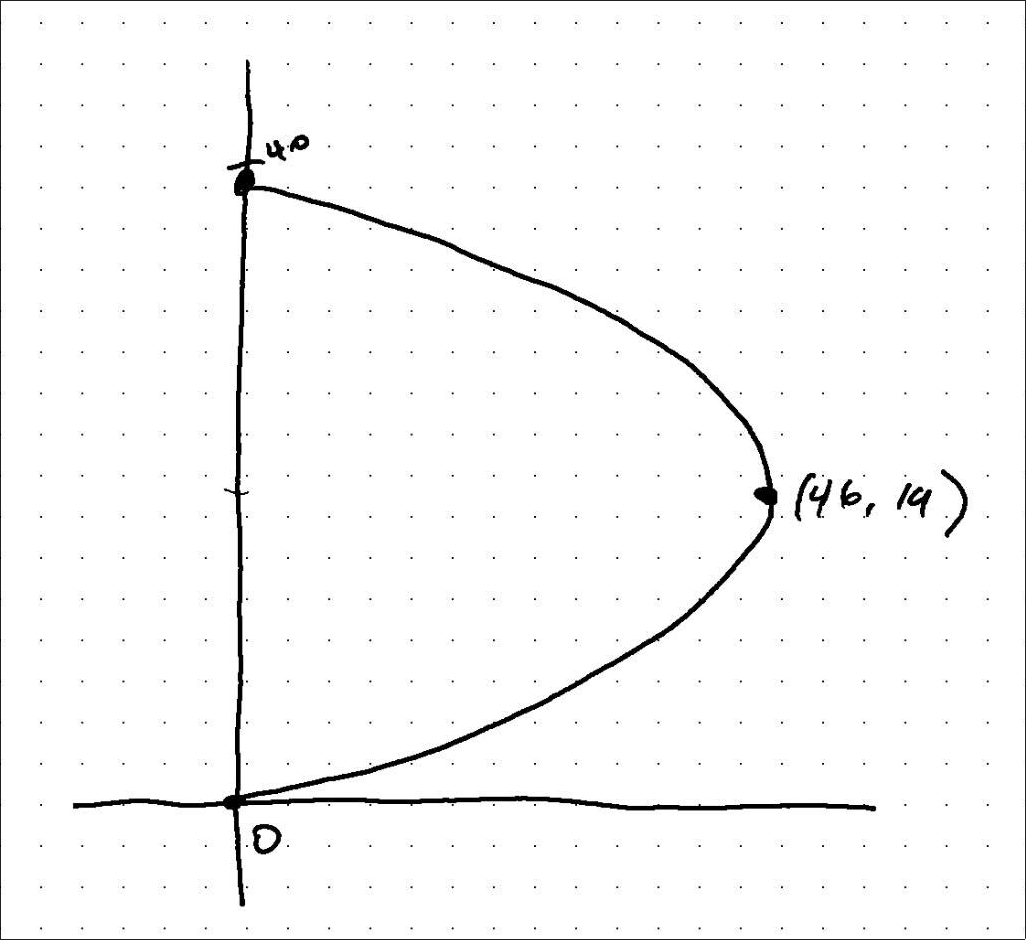
\includegraphics[scale=0.2]{graph-1.png}
\end{figure}

\section*{Problem 7}
The angular position of a rod varies as 20.0$t^2$ radians starting from time $t = 0$ . The rod has
two beads on it as shown in the following figure, one at 10.0 cm from the rotation axis and the
other at 20.0 cm from the rotation axis. (a) What is the instantaneous angular velocity of the rod
at $t = 5.00$ s? (b) What is the angular acceleration of the rod? (c) What are the tangential speeds
of the beads at $t$ = 5.00 s? (d) What are the tangential accelerations of the beads at $t$ = 5.00 s? (e)
What are the centripetal accelerations of the beads at $t$ = 5.00 s?

\begin{figure}[ht]
    \centering
    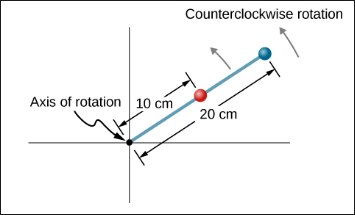
\includegraphics[scale=0.5]{drawing-2.png}
\end{figure}

\subsection*{Solution}
\subsubsection*{Part a:}
If angular position is given by
\begin{equation}
	\theta(t) = 20t^2
\end{equation}
then the angular velocity is;
\[
\theta^\prime(t) = 40t \big\rvert_{t=5} = \boxed{200\ \text{rad}/\text{s}}
\]

\subsubsection*{Part b:}
\[
	\theta^{\prime\prime}(t) = \boxed{40\ \text{rad}/\text{s}^2}
\]

\subsubsection*{Part c:}
The tangential speed is given by
\[
	v_t = \omega r
\]
therefore, for the 10 cm bead;

\[
	v_{t,10} = 200 \cdot 10 = \boxed{2000\ \text{cm}/\text{s}}
\]
and for the 20 cm bead;

\[
	v_{t,20} = 200 \cdot 20 = \boxed{4000\ \text{cm}/\text{s}}
\]

\subsubsection*{Part d:}
Similarly, the tangential acceleration is

\[
	a_t = \alpha r
\]
so we have;

\[
	a_{r,10} = 40 \cdot 10 = \boxed{400\ \text{cm}/\text{s}^2}
\]
and

\[
	a_{r,20} = 40 \cdot 20 = \boxed{800\ \text{cm}/\text{s}^2}
\]

\subsubsection*{Part e:}
The centripetal acceleration is

\[
	a_c = \frac{v^2}{r}
\]
so we have

\[
	a_{c,10} = \frac{2000^2}{10} = \boxed{400\ 000\ \text{cm}/\text{s}^2}
\]
and

\[
	a_{c,20} = \frac{4000^2}{20} = \boxed{800\ 000\ \text{cm}/\text{s}^2}
\]

\section*{Problem 8}
The angular acceleration of a rotating rigid body is given by $\alpha = (A-Bt)$, where $A$ =
2.00 rad/s$^2$ and $B$ = 3.00 rad/s$^3$. If the body starts rotating from rest at $t$ = 0 , (a) what is the angular
velocity? (b) Angular position? (c) What angle does it rotate through in 10.0 s? (d) Where does
the vector perpendicular to the axis of rotation indicating 0$^\circ$ at $t$ = 0 lie at $t$ = 10.0 s ?

\subsection*{Solution}
\subsubsection*{Part a:}
Given the angular acceleration equation we can integrate to find the angular velocity function;
\begin{align*}
	\int d\omega &= \int (A - Bt) \ dt \\
	\omega(t) &= At - \frac{Bt^2}{2} + C \\
	\omega(t) &= At - \frac{Bt^2}{2}\\
	\omega(t) &= 2.00t - 1.50 t^2\ \text{rad}/\text{s}
\end{align*}

\subsubsection*{Part b:}
We can integrate the velocity function to find the position function;
\begin{align*}
	\int d\theta &= \int (2.00t - 1.50t^2) \ dt \\
	\theta(t) &= t^2 - \frac{1.50 t^3}{3} + C \\
	\theta(t) &= t^2 - \frac{1}{2}t^3 \ \text{rad}
\end{align*}

\subsubsection*{Part c:}
\[
	\theta(10.0) = 10^2 - \frac{1}{2}10^3 = \boxed{-400\ \text{rad}}
\]

\subsubsection*{Part d:}
We start by converting the radians to degrees
\[
	-400 \cdot \frac{180}{\pi} = -22\ 918.31
\]
then find the number of times the degrees goes into one full revolution
\[
	n = \Biggr\lceil \frac{22\ 918.31}{360} \Biggr\rceil = 64
\]
then

\[
	\theta = -22\ 918.31 + 23\ 040 = \boxed{121.69^\circ}
\]

\end{document}
